\section{Durchführung}
In Abbildung~\ref{fig:resonatoren} sind die verwendeten Bauteile der Röhren- und Hohlraummresonatoren und die Halterung für den Röhrenresonator zu sehen.

\begin{figure}[H]
  \centering
  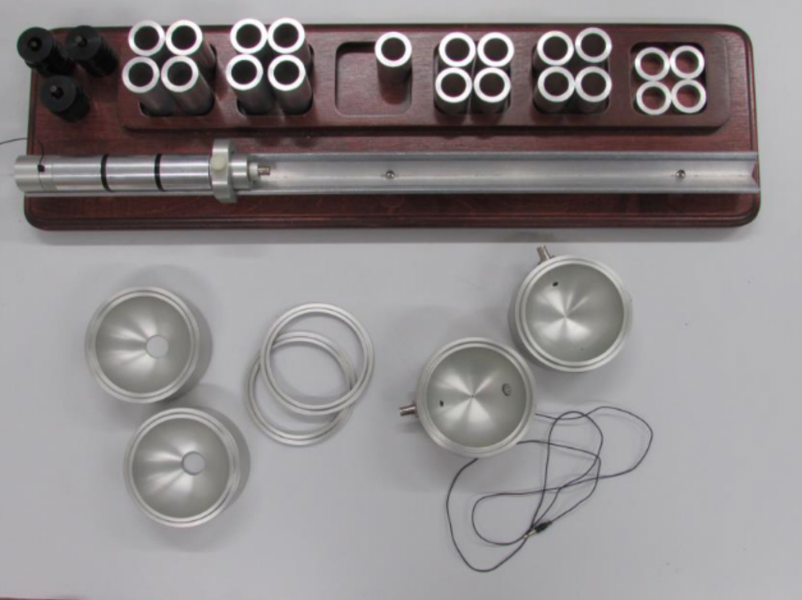
\includegraphics[width=12cm, keepaspectratio]{resonatoren.png}
  \caption{Bestandteile der verwendeten Röhren- und Kugelresonatoren \cite{anleitung}.}
  \label{fig:resonatoren}
\end{figure}

In jedem Teilversuch wird die Schalldruckamplitude als Funktion der Frequenz untersucht. Dies erfolgt entweder über ein eigens dafür entworfenes Programm, oder über einen Sinusgenerator und ein Oszilloskop. Für den letzteren Fall ist in Abbdildung~\ref{fig:schaltskizze} die Schaltskizze zu sehen.

\begin{figure}[H]
  \centering
  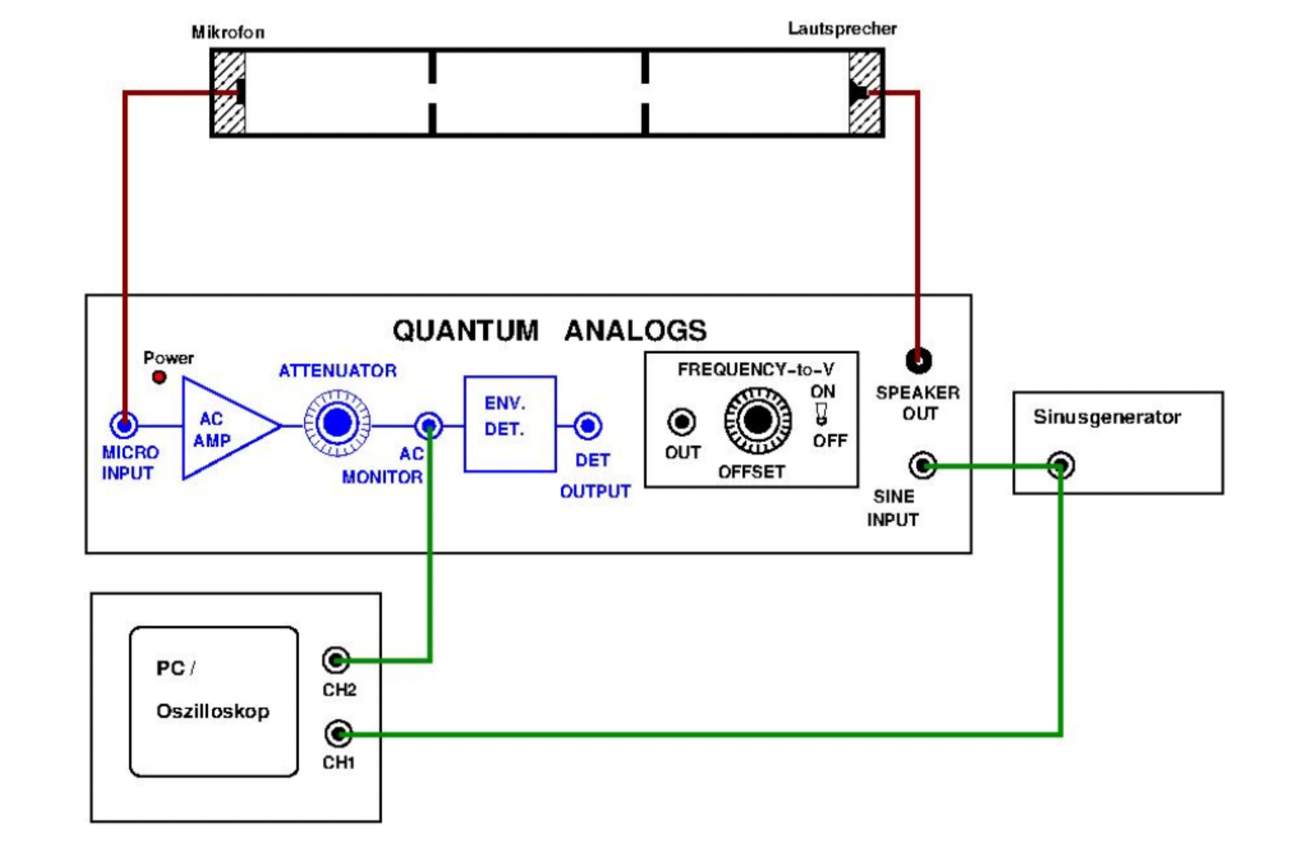
\includegraphics[width=12cm,keepaspectratio]{schaltskizze.png}
  \caption{Schaltskizze zur Messung der Eigenmoden im Resonator mit einem Oszilloskop \cite{anleitung}.}
  \label{fig:schaltskizze}
\end{figure}

\subsection{Vorbereitende Messungen}
Zur Vorbereitung werden die Frequenzspektren von Röhrenresonatoren bestehend aus $\SI{50}{\mm}$-Zylindern von $\SI{0.1}{\kilo\hertz}$ bis $\SI{12}{\kilo\hertz}$ aufgenommen. Dies wird für Röhrenresonatoren bestenend aus $1$--$12$ Resonatoren zunächst mit dem 2-Kanal-Oszilloskop und daraufhin mit dem PC getan. Bei Verwendung des Sinus-Generators wird die Sweep-Dauer auf $\SI{30}{\second}$ gestellt. Daraufhin wird auch das Frequenzspektrum eines $\SI{75}{\mm}$-Zylinders mit dem PC aufgenommen.

\subsection{Das H-Atom}
Für diesen Versuchsteil wird ein Hohlraumresonator bestehend aus einer Hälfte mit einem Mikrofon und einer Hälfte mit einem Lautsprecher an den PC angeschlossen. Zunächst wird ein hochaufgelöstes Frequenzspektrum, also $\SI{50}{\hertz}$-Schritte mit $\SI{60}{\milli\second}$ pro Schritt, im Bereich $\SIrange{0.1}{12}{\kilo\hertz}$ aufgenommen, wobei sich Lausprecher und Mikrofon genau gegenüberstehen. Daraufhin werden am 2-Kanal-Oszilloskop Frequenz, Amplitude und Phasenverschiebung beobachtet, während der Sinusgenerator den Frequenzbereich von $\SI{100}{\hertz}$ bis $\SI{10}{\kilo\hertz}$ durchläuft. Dabei werden ausgewählte Resonanzfrequenzen und die dazugehörige Ordnung notiert.

Weiterhin werden hochaufgelöste Frequenzspektren als Funktion des Drehwinkels zwischen Lautsprecher und Mikrofon aufgenommen. Dies geschieht in $\SI{10}{\degree}$-Schritten in einem Bereich von $\SI{0}{\degree}$ bis $\SI{180}{\degree}$.

Außerdem wird bei einem Winkel von $\SI{180}{\degree}$ zwischen Mikrofon und Lautsprecher ein Frequenzspektrum im Bereich $\SIrange{1.8}{2.6}{\kilo\hertz}$ mit $\SI{1}{\hertz}$-Schritten und $\SI{60}{\milli\second}$ pro Schritt für Zwischenringe der Dicke $\num{3}$, $\num{6}$ und $\SI{9}{\milli\metre}$ aufgenommen.

Zuletzt werden mit einem $\SI{9}{\milli\metre}$-Zwischenring Spektren im selben Frequenzbereich unter Variation des Winkels aufgenommen. Hierbei wird der Winkel wieder im Bereich $\SIrange{0}{180}{\degree}$ in $\SI{10}{\degree}$-Schritten variiert.

\subsection[Das $\mathrm{H}_2^{+}$-Molekül]{Das $\symbf{\mathrm{H}_2^{+}}$-Molekül}
In diesem Versuchteil wird das akustische Modell des $\mathrm{H}_2^+$-Moleküls, also zwei gekoppelte Kugelresonatoren, untersucht. Hierzu wird zunächst das Frequenzspektrum im Bereich $\SIrange{2.2}{2.5}{\kilo\hertz}$ mit $\SI{1}{\hertz}$-Schritten und $\SI{75}{\milli\second}$ pro Schritt mit verschiedenen Blenden zwischen den beiden Hohlraumresonatoren aufgenommen. Die verwendeten Blendendurchmesser sind $\SIlist{5;10;15;20}{\milli\metre}$ und der Winkel zwischen Mikrofon und Lautsprecher beträgt $\SI{180}{\degree}$.

Außerdem werden unter Verwendung der $\SI{15}{\milli\metre}$-Blende in einem Winkelbereich von $\SI{0}{\degree}$ bis $\SI{180}{\degree}$ in $\SI{10}{\degree}$-Schritten Frequenzspektren im selben Frequenzbereich wie zuvor aufgenommen.

Zuletzt wird die Phasenverschiebung der Druckamplitude in der unteren und der oberen Kugel für alle Resonanzfrequenzen im untersuchten Frequenzbereich bei einem Winkel von $\SI{180}{\degree}$ aufgenommen. Dies geschieht mit dem 2-Kanal-Oszilloskop.

\subsection{Der eindimensionale Festkörper}
In diesem Teilversuch wird wieder der Röhrenresonator verwendet und jegliche Frequenzspektren werden mit dem PC aufgenommen.

Zunächst wird das Frequenzspektrum eines Röhrenresonators bestehend aus zwei $\SI{50}{\milli\metre}$-Zylindern und einer Irisblende mit einem Durchmesser von $\SI{16}{\milli\metre}$ zwischen den beiden Zylindern in einem Frequenzbereich von $\SI{0.1}{\kilo\hertz}$ bis $\SI{12}{\kilo\hertz}$ mit $\SI{5}{\hertz}$-Schritten und $\SI{50}{\milli\metre}$ pro Schritt aufgenommen. Der Röhrenresonator wird jeweils um eine Irisblende und einen Zylinder ergänzt und für jede Ergänzung wird das Frequenzspektrum erneut aufgenommen bis zehn Zylinder verbaut sind.
Diese Messung wird wiederholt mit zwei, vier, und zehn Zylindern mit $\SI{10}{\milli\metre}$ bzw. $\SI{13}{\milli\metre}$-Blenden dazwischen.

Daraufhin wird das Frequenzspektrum für einen Röhrenresonator bestehend aus zehn $\SI{50}{\milli\metre}$-Zylindern und $\SI{16}{\milli\metre}$-Blenden dazwischen aufgenommen, wobei einer der Zylinder ersetzt wird durch einen Zylinder der Länge $\SI{75}{\milli\metre}$. Diese Messung wird wiederholt mit einem Zylinder der Länge $\SI{62.5}{\milli\metre}$ und $\SI{37.5}{\milli\metre}$.

Weiterhin wird das Frequenzspektrum eines Röhrenresonators bestehend aus zehn Zylindern gekoppelt durch $\SI{16}{\milli\metre}$-Blenden, wobei die Zylinder abwechselnd $\SI{50}{\milli\metre}$ und $\SI{75}{\milli\metre}$ lang sind.

Zuletzt wird das Frequenzspektrum eines Röhrenresonators aus acht $\SI{50}{\milli\metre}$ langen Zylindern mit Irisblenden dazwischen aufgenommen, wobei die Blendendurchmesser abwechselnd $\SI{13}{\milli\metre}$ und $\SI{16}{\milli\metre}$ betragen.
